\subsection{Homogeneous Multicore Systems}
%\begin{figure}[t]%
%    \label{fig:speedup_homo}
%	\centering
%	%\begin{subfigure}
%	\subfloat [] 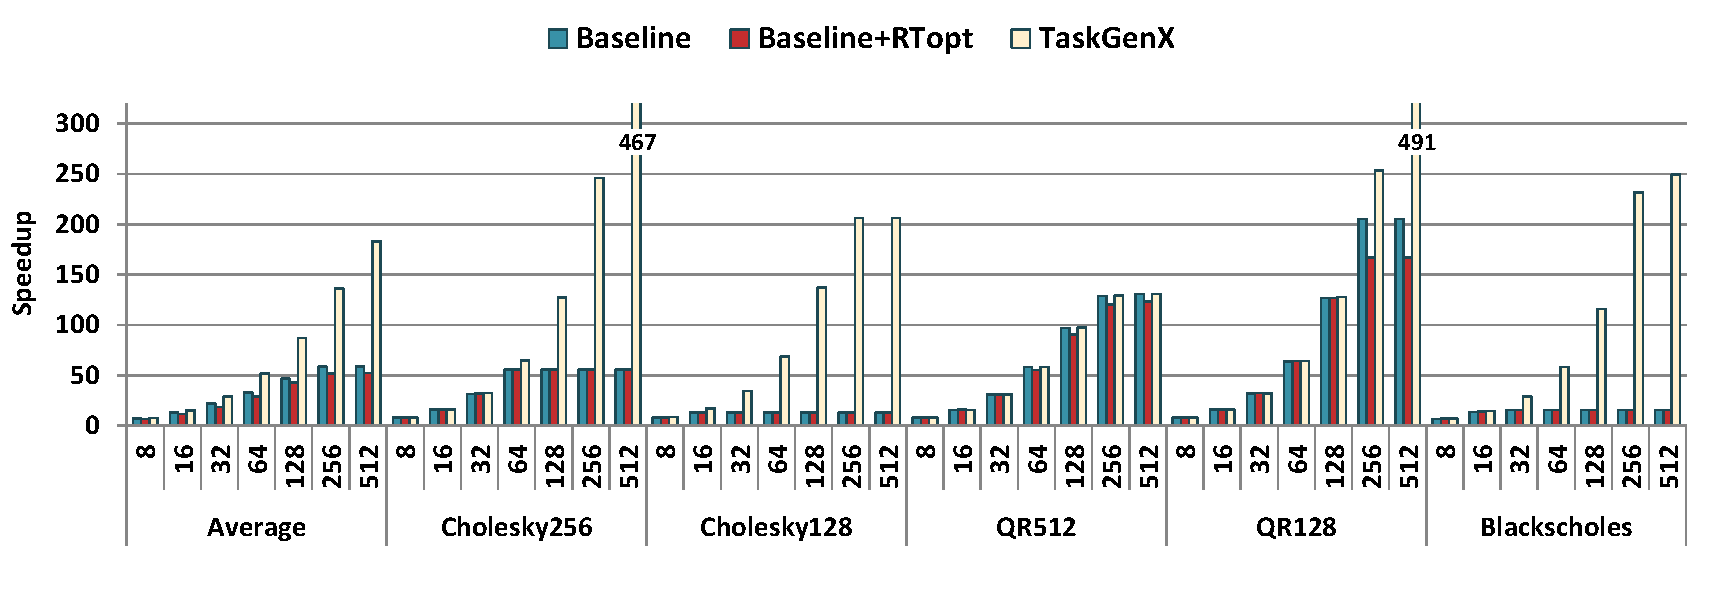
\includegraphics[width=1.0\textwidth]{figures/speedup_homo.pdf}
%	%\caption{test}
%	%\end{subfigure}
%	%\begin{subfigure}
%	\subfloat [] 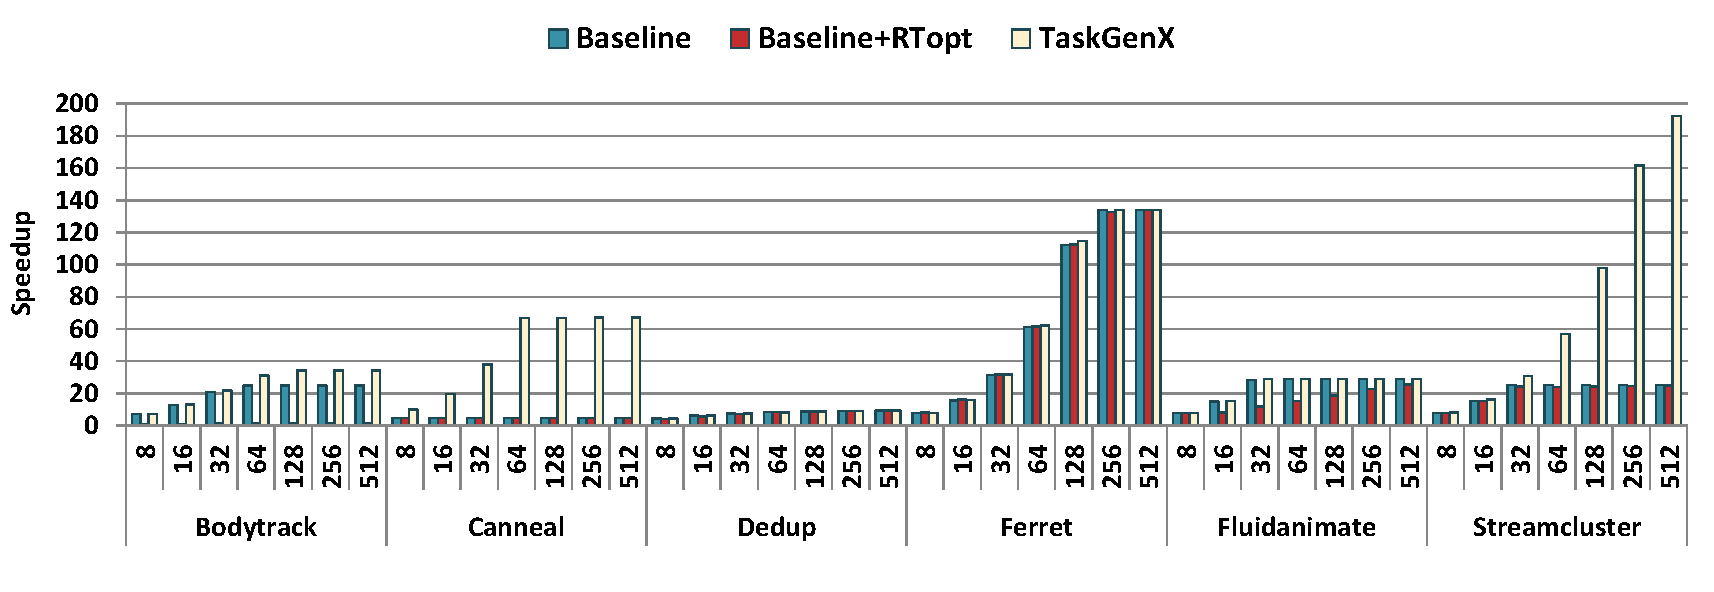
\includegraphics[width=1.0\textwidth]{figures/speedup_homo2.pdf}
%	%\end{subfigure}
%	\vspace{-0.5cm}
%	\caption{Communication mechanism between master/workers and SRT threads.}
%	\vspace{-0.3cm}
%\end{figure}

\begin{figure}[t]%
	\centering
	\subfloat[]{\label{fig:speedup_homo1}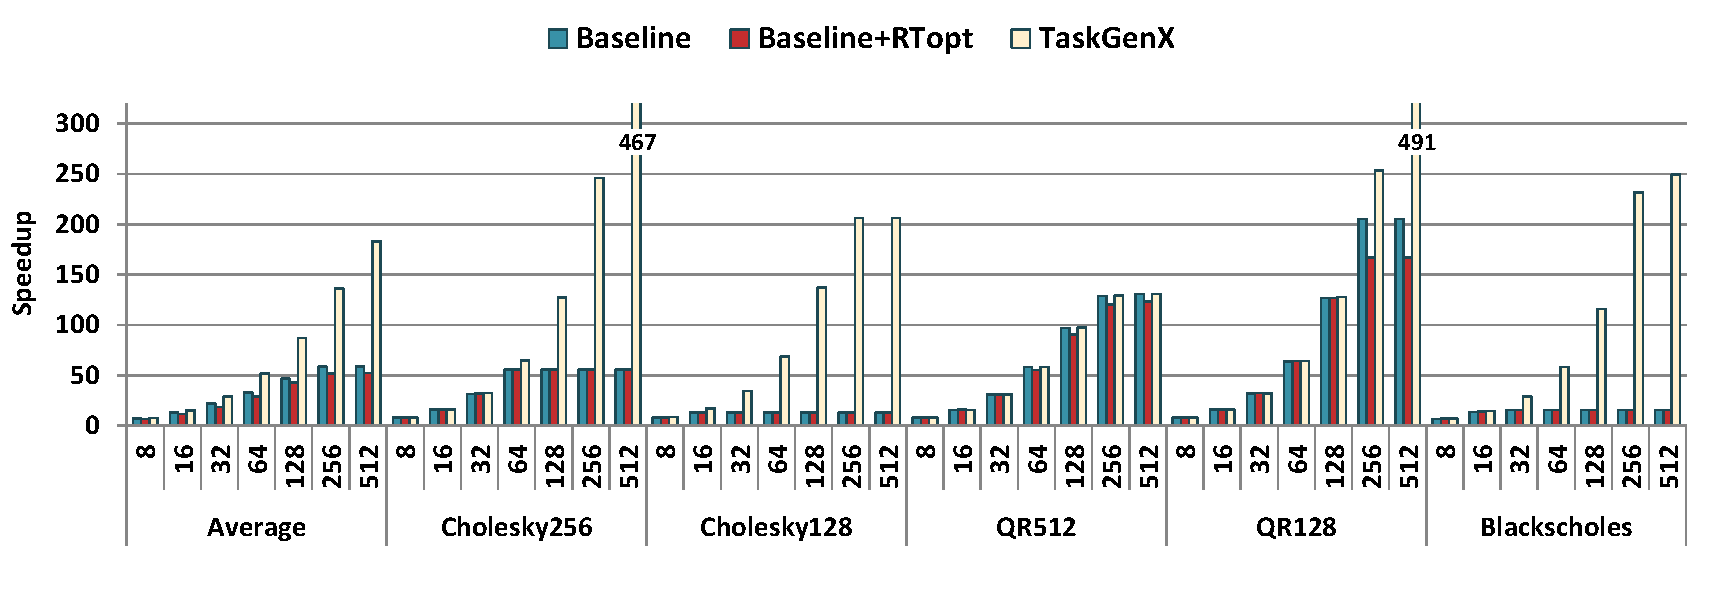
\includegraphics[width=\columnwidth]{figures/speedup_homo.pdf}}
	
	\subfloat[]{\label{fig:speedup_homo2}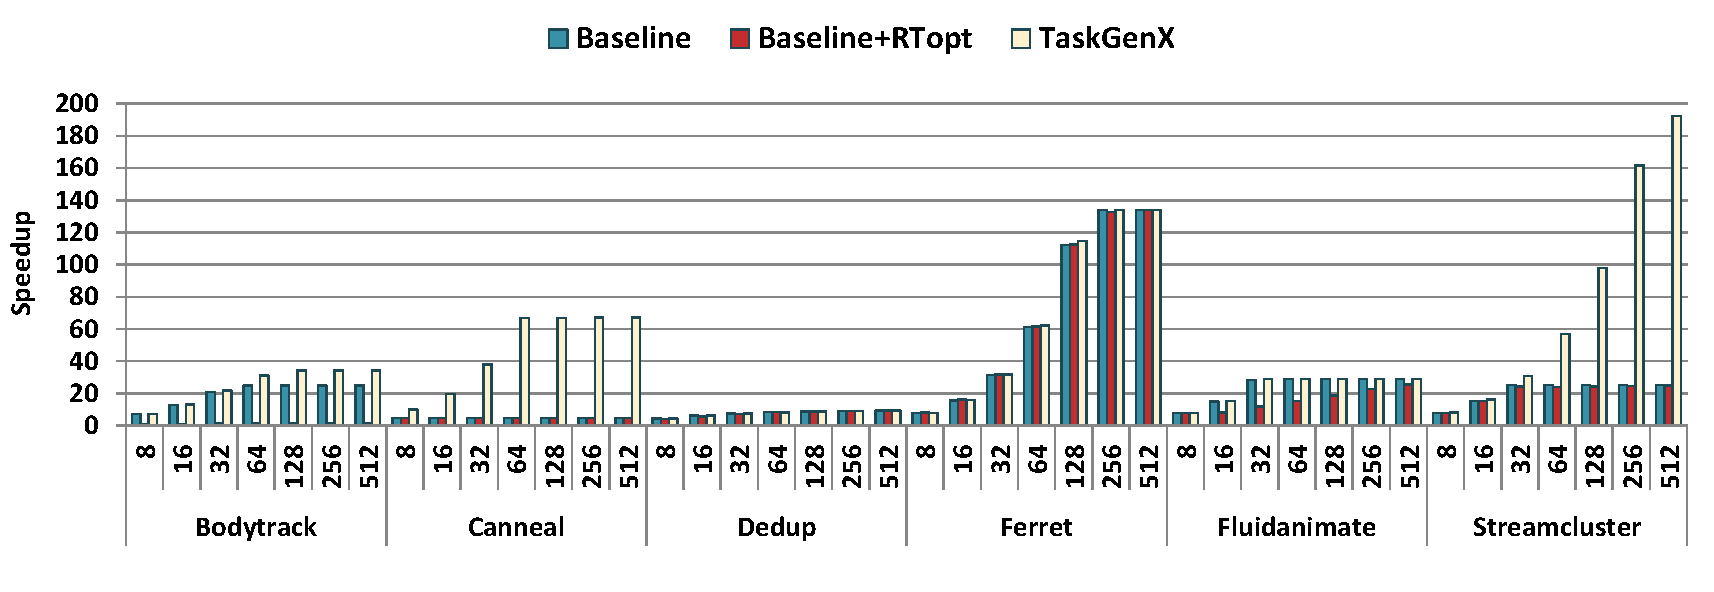
\includegraphics[width=\columnwidth]{figures/speedup_homo2.pdf}}
	\caption{Speedup of {\proposal} compared to the speedup of Baseline and Baseline+RTopt for each application for systems with 8 up to 512 cores. The average results of (a) show the average among all workloads shown on (a) and (b)}
\end{figure}

Figures~\ref{fig:speedup_homo1} and~\ref{fig:speedup_homo2} show the speedup over one core of three different scenarios: 
\begin{itemize}
\item \textit{Baseline}: the Nanos++ runtime system, which is the default runtime without using any external hardware support
\item \textit{Baseline+RTopt}: the Nanos++ runtime system that uses the external hardware as if it is a general purpose core 
\item \textit{{\proposal}}: our proposed runtime system that takes advantage of the optimized hardware
\end{itemize}
We evaluate these approaches with the TaskSim simulator for systems of 8 up to 512 cores.
In the case of Baseline+RTopt the specialized hardware acts as a slow general purpose core that is additional to the number of cores shown on the x axis.
If this core executes a task creation job, it executes it 16$\times$ faster, but as it is specialized for this, we assume that when a task is executed on this core it is executed 4$\times$ slower than in a general purpose core.
The runtime system in this case does not include our modifications that automatically decouple the task creation step for each task.
The comparison against the Baseline+RTopt is used only to show that the baseline runtime is not capable of effectively utilizing the accelerator. 
In most of the cases having this additional hardware without the appropriate runtime support results in slowdown as the tasks are being executed slower on the special hardware.

Focusing on the average results first, we can observe that {\proposal} constantly improves the baseline and the improvement is increasing as the number of cores is increased, reaching up to 3.1$\times$ improved performance on 512 cores. 
This is because as we increase the number of cores, the task creation overhead becomes more critical part of the execution time and affects performance even more.
So, this becomes the main bottleneck due to which the performance of many applications saturates. 
{\proposal} overcomes it by automatically detecting and moving task creation on the specialized hardware.

Looking in more detail, we can see that for all applications the baseline has a saturation point in speedup.
For example Cholesky256 saturates on 64 cores, while QR512 on 256 cores.
In most cases this saturation in performance comes due to the sequential task creation that is taking place for an important percentage of the execution time (as shown in Figure~\ref{fig:master_thread}).
{\proposal} solves this as it efficiently decouples the task creation code and accelerates it leading to higher speedups.

{\proposal} is effective as it either improves performance or it performs as fast as the baseline (there are no slowdowns). 
The applications that do not benefit (QR512, Ferret, Fluidanimate) are the ones with the highest average per task CPU cycles as shown on Table~\ref{tab.apps}.
Dedup also does not benefit as the per task creation cycles are very low compared to its average task size.
Even if these applications consist of many tasks, the task creation overhead is considered negligible compared to the task cost, so accelerating it does not help much. 
%\begin{figure*}[!t]
%\centering

%\begin{figure}[b]
%\begin{tabular}{@{}c@{}}
%  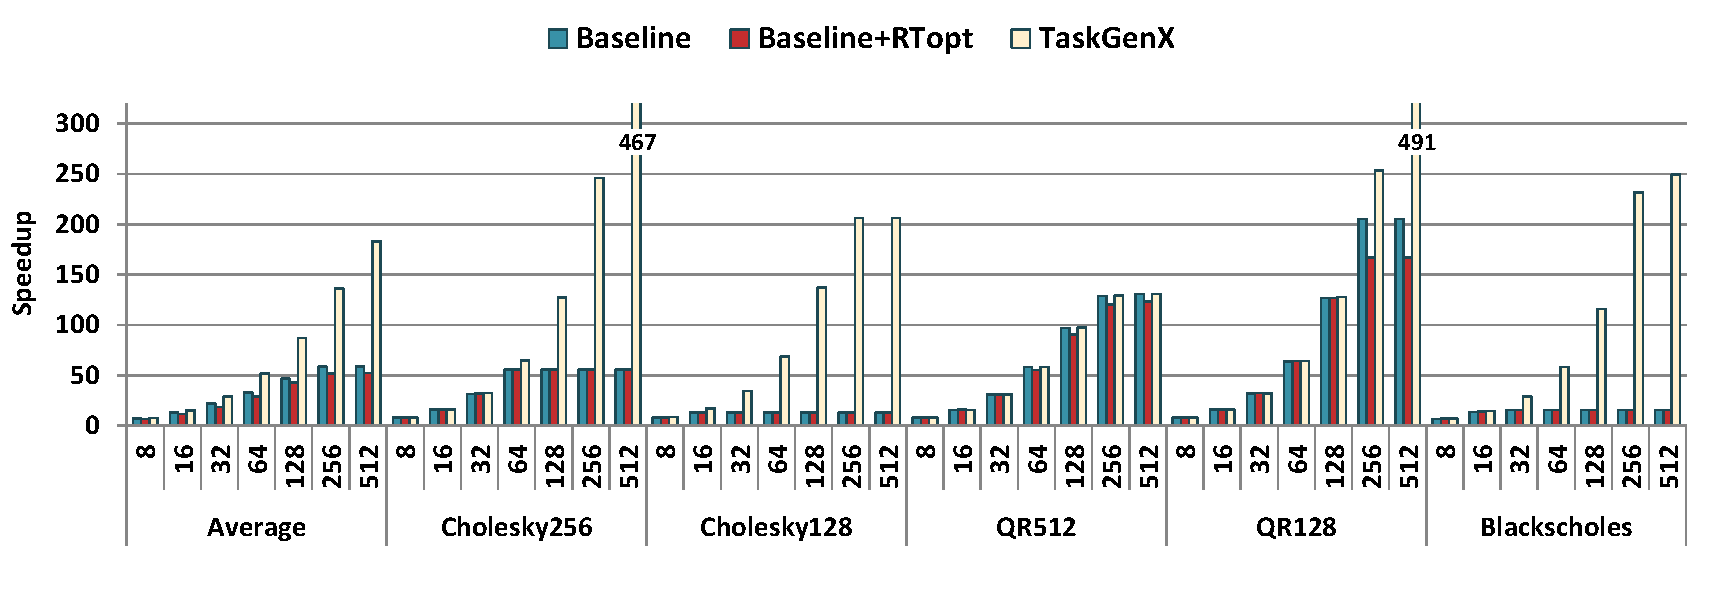
\includegraphics[width=\textwidth]{figures/speedup_homo.pdf}
%  \caption{}
%  \label{fig:speedup_homo1}
%\end{figure}
%
%\begin{figure}[b]
%  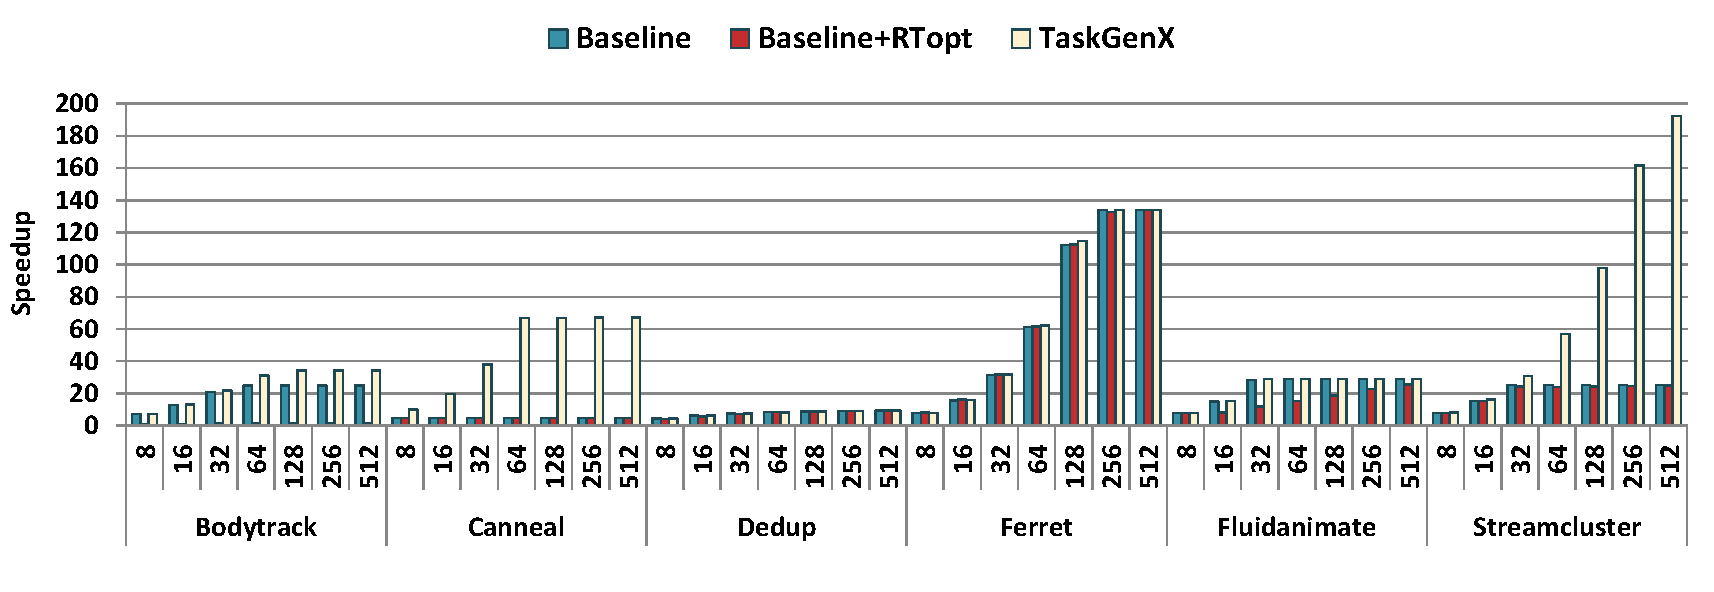
\includegraphics[width=\textwidth]{figures/speedup_homo2.pdf}
%  \caption{}
%  \label{fig:speedup_homo2}
%\end{figure}


This can be verified by the results shown for QR128 workload.
In this case, we use the same input size as QR512 (which is 16K) but we modify the block size, which results in more and smaller tasks.
This not only increases the speedup of the baseline, but also shows even higher speedup when running with {\proposal} reaching very close to the ideal speedup and improving the baseline by 2.3$\times$.
%\begin{figure*}[t]%
%	\centering
%	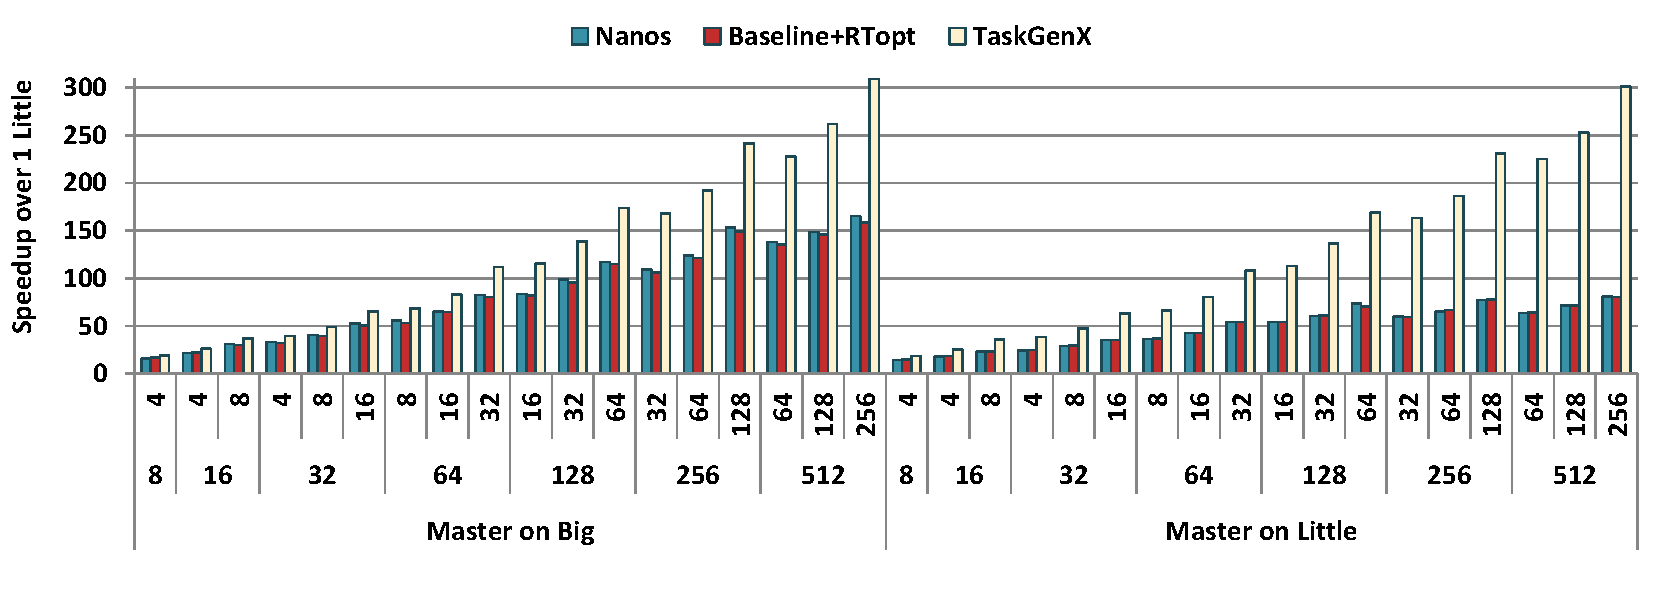
\includegraphics[width=\textwidth]{figures/speedup_hetero_avg.pdf}
%	\caption{Average speedup among all 11 workloads on heterogeneous simulated systems. The numbers at the bottom of x axis show the total number of cores and the numbers above them show the number of big cores. Results are separated depending on the type of core that executes the master thread: a big or little core.}
%	\label{fig:hetero}%
%	\vspace{-0.3cm}
%\end{figure*}
%\begin{figure}[t]%
%	\centering
%	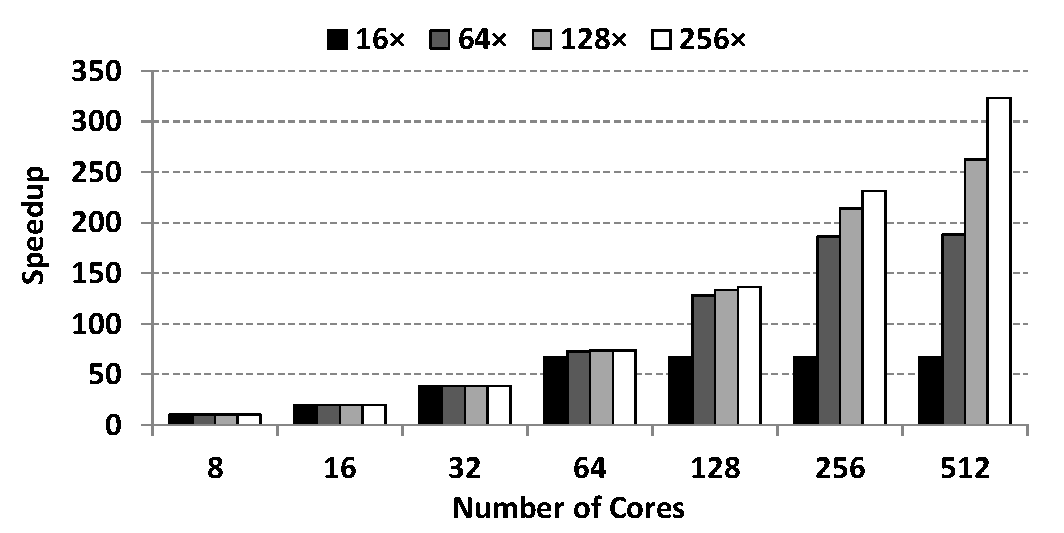
\includegraphics[width=0.6\columnwidth]{figures/canneal_perf.pdf}
%	\caption{Canneal performance as we modify $r$ }
%	\label{fig:canneal}%
%\end{figure}
\begin{figure}[t]
	\centering
	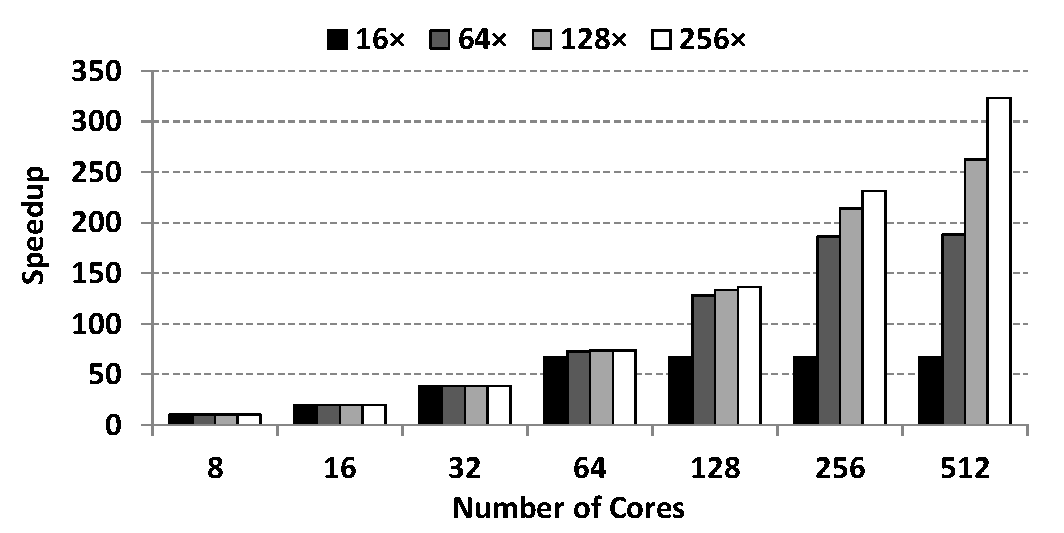
\includegraphics[width=0.75\columnwidth]{figures/canneal_perf.pdf}
	\caption{Canneal performance as we modify $r$; $x$-axis shows the number of cores.}
	\label{fig:canneal}
\end{figure}
Modifying the block size for Cholesky, shows the same effect in terms of {\proposal} over baseline improvement.
However, for this application, using the bigger block size of 256 is more efficient as a whole.
Nevertheless, {\proposal} improves the cases that performance saturates and reaches up to 8.5$\times$ improvement for the 256 block-size, and up to 16$\times$ for the 128 block-size.

Blackscholes and Canneal, are applications with very high task creation overheads compared to the task size as shown on Table~\ref{tab.apps}.
This makes them very sensitive to performance degradation due to task creation. 
As a result their performance saturates even with limited core counts of 8 or 16 cores.
These are the ideal cases for using {\proposal} as such bottlenecks are eliminated and performance is improved by 15.9$\times$ and 13.9$\times$ respectively.
However, for Canneal for which the task creation lasts a bit less than half of the task execution time, accelerating it by 16 times is not enough and soon performance saturates at 64 cores. 
In this case, a more powerful hardware would improve things even more.
Figure~\ref{fig:canneal} shows how the performance of Canneal is affected when modifying the task creation performance ratio, $r$ between the specialized hardware and general purpose.
Using hardware that performs task creation close to 256$\times$ faster than the general purpose core leads to higher improvements.

Streamcluster has also relatively high task creation overhead compared to the average task cost so improvements are increased as the number of cores is increasing.
{\proposal} reaches up to 7.6$\times$ improvement in this case.

The performance of Bodytrack saturates on 64 cores for the baseline. 
However, it does not approach the ideal speedup as its pipelined parallelization technique introduces significant task dependencies that limit parallelism.
{\proposal} still improves the baseline by up to 37\%.
This improvement is low compared to other benchmarks, firstly because of the nature of the application and secondly because Bodytrack introduces nested parallelism.
With nested parallelism task creation is being spread among cores so it is not becoming a sequential overhead as happens in most of the cases.
Thus, in this case task creation is not as critical to achieve better results.
%correct to look at the CREATE overhead value as this is be parallelized among all cores for the 329\,123 tasks of the application. 


\subsection{Heterogeneous Multicore Systems}

%\begin{figure}[t]%
%	\centering
%	\subfloat[Average speedup among all 11 workloads on heterogeneous simulated systems. The numbers at the bottom of x axis show the total number of cores and the numbers above them show the number of big cores. Results are separated depending on the type of core that executes the master thread: a big or little core.]{\label{fig:hetero}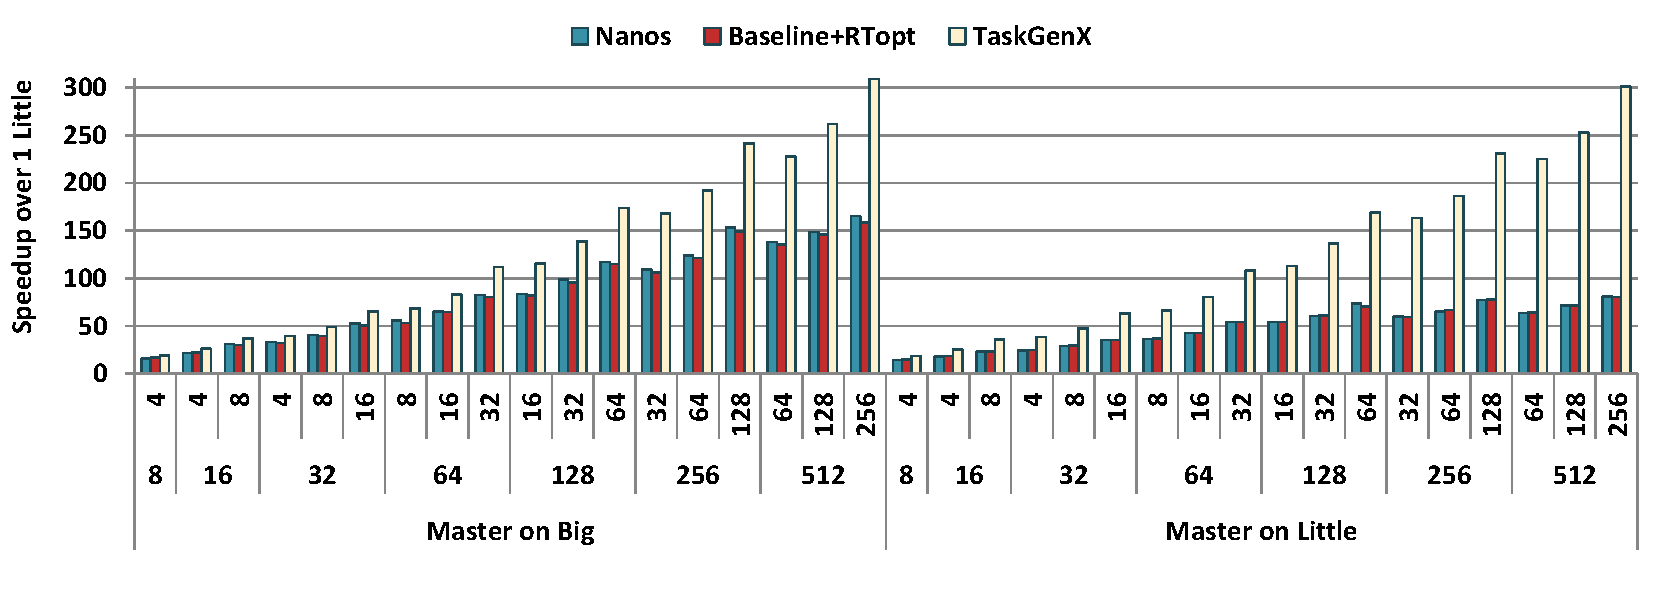
\includegraphics[width=\columnwidth]{figures/speedup_hetero_avg.pdf}}
%	
%	\subfloat[Canneal performance as we modify $r$]{\label{fig:canneal}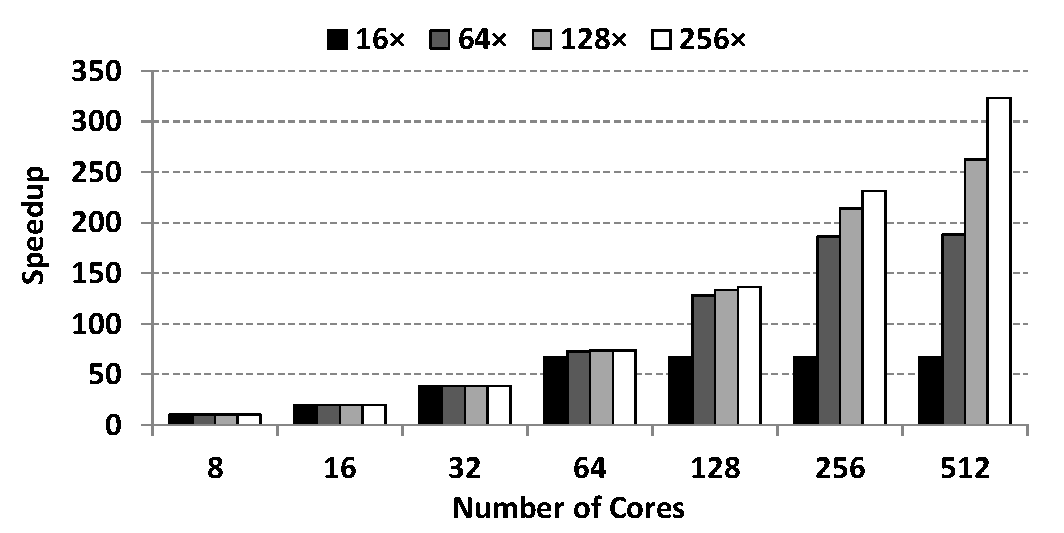
\includegraphics[width=0.5\columnwidth]{figures/canneal_perf.pdf}}
%\subfloat[Average improvement over baseline]{\label{fig:baseline}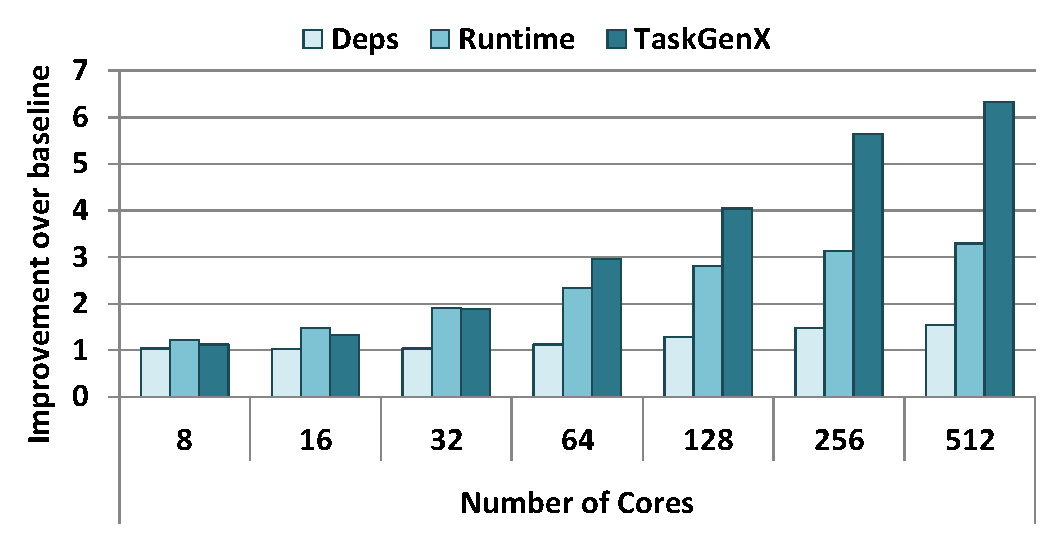
\includegraphics[width=0.48\textwidth]{figures/comparison.pdf}}
%	\vspace{-0.3cm}
%	\caption{X-axis of Figures \ref{fig:canneal} and \ref{fig:baseline} shows the number of cores. For each case an RTopt core is used additionally to the number of cores.}
%\end{figure}

\begin{figure*}[t]%
	\centering
	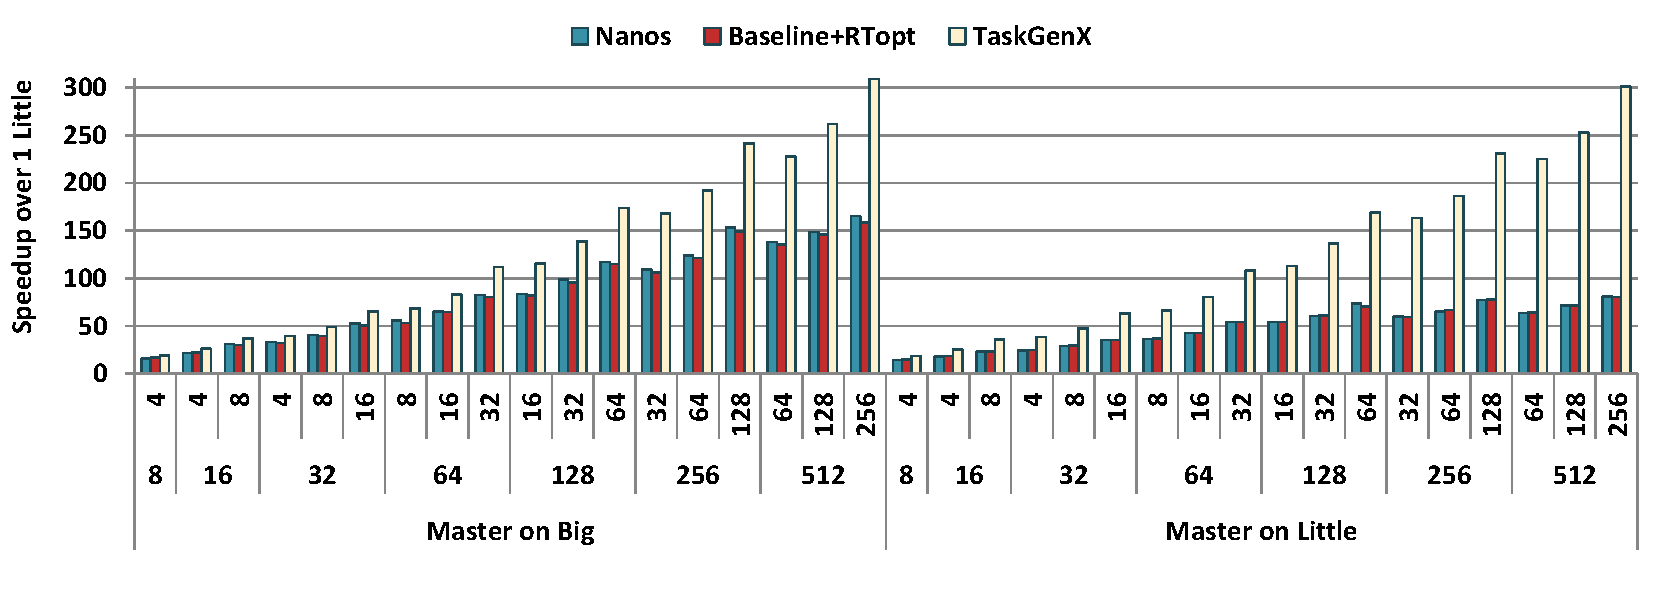
\includegraphics[width=\columnwidth]{figures/speedup_hetero_avg.pdf}
	\caption{Average speedup among all 11 workloads on heterogeneous simulated systems. The numbers at the bottom of x axis show the total number of cores and the numbers above them show the number of big cores. Results are separated depending on the type of core that executes the master thread: a big or little core.}	
	\label{fig:hetero}
\end{figure*}


%	\subfloat[Canneal performance as we modify $r$]{\label{fig:canneal}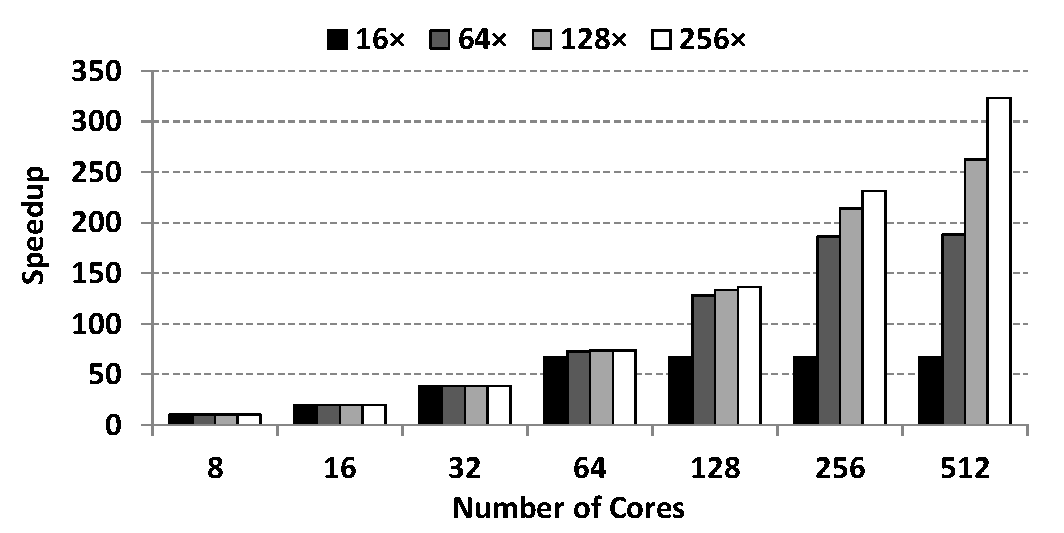
\includegraphics[width=0.5\columnwidth]{figures/canneal_perf.pdf}}
%\subfloat[Average improvement over baseline]{\label{fig:baseline}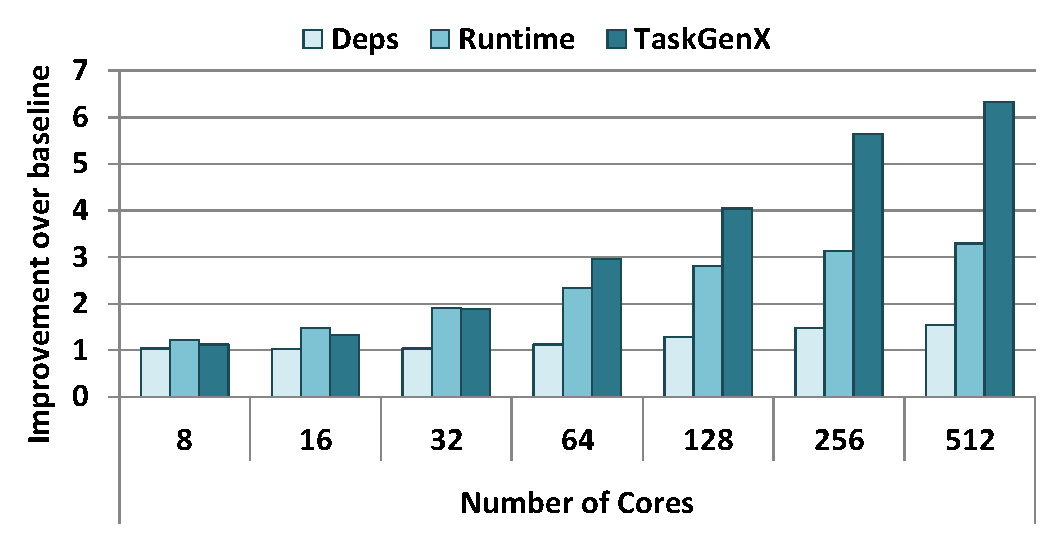
\includegraphics[width=0.48\textwidth]{figures/comparison.pdf}}
%	\vspace{-0.3cm}
%	\caption{X-axis of Figures \ref{fig:canneal} and \ref{fig:baseline} shows the number of cores. For each case an RTopt core is used additionally to the number of cores.}
%\end{figure}


%Figure~\ref{fig:hetero} shows the average speedup obtained among the same applications. 
At this stage of the evaluation our system supports two types of general purpose processors, simulating an asymmetric multi-core processor.
The asymmetric system is influenced by the ARM big.LITTLE architecture~\cite{ARM} that consists of big and little cores.
In our simulations, we consider that the big cores are four times faster than the little cores of the system.
This is based on the average measured performance ratio, shown on Table~\ref{tab.apps}, among the 11 workloads used in this evaluation.
%This assumption is based on prior works~\cite{Chronaki:TPDS} that have shown that for most applications the performance ratio ranges from 3.5$\times$ to 4.5$\times$.

In this set-up there are two different ways of executing a task-based application.
The first way is to start the application's execution on a big core of the system and the second way is to start the execution on a little core of the system.
If we use a big core to load the application, then this implies that the master thread of the runtime system (the thread that performs the task creation when running with the baseline) runs on a fast core, thus tasks are created faster than when using a slow core as a starting point.
We evaluate both approaches and compare the results of the baseline runtime and {\proposal}.

Figure~\ref{fig:hetero} plots the average speedup over one little core obtained among all 11 workloads for the Baseline, Baseline+RTopt and {\proposal}.
The chart shows two categories of results on the x axis, separating the cases of the master thread's execution.
The numbers at the bottom of x axis show the total number of cores and the numbers above show the number of big cores.

%The bars represent the average speedup when running with the baseline runtime or with {\proposal} and the line shows the ideal speedup for each configuration.
%The ideal speedup is the speedup that we would obtain if we were running an application in parallel assuming zero runtime overheads and no dependencies between tasks, technically unachievable for the real applications of our evaluation.
%Equation~\ref{eq.ideal} shows how the ideal speedup is computed for our simulated system where the big cores are four times faster than the little cores.
%\begingroup\makeatletter\def\f@size{9}\check@mathfonts
%\begin{equation}
%  \text{$ideal\_speedup(big, little) = big \times 4 + little$}
%\label{eq.ideal}
%\end{equation}
%\endgroup

The results show that moving the master thread from a big to a little core degrades performance of the baseline.
This is because the task creation becomes even slower so the rest of the cores spend more idle time waiting for the tasks to become ready.
{\proposal} improves performance in both cases.
Specifically when master runs on big, the average improvement of {\proposal} reaches 86\%.
When the master thread runs on a little core, {\proposal} improves performance by up to 3.7$\times$. 
This is mainly due to the slowdown caused by the migration of master thread on a little core.
Using {\proposal} on asymmetric systems achieves approximately similar performance regardless of the type of core that the master thread is running. 
This makes our proposal more portable for asymmetric systems as the programmer does not have to be concerned about the type of core that the master thread migrates.

\subsection{Comparison to Other Approaches}
\begin{figure}[t]
	\centering
	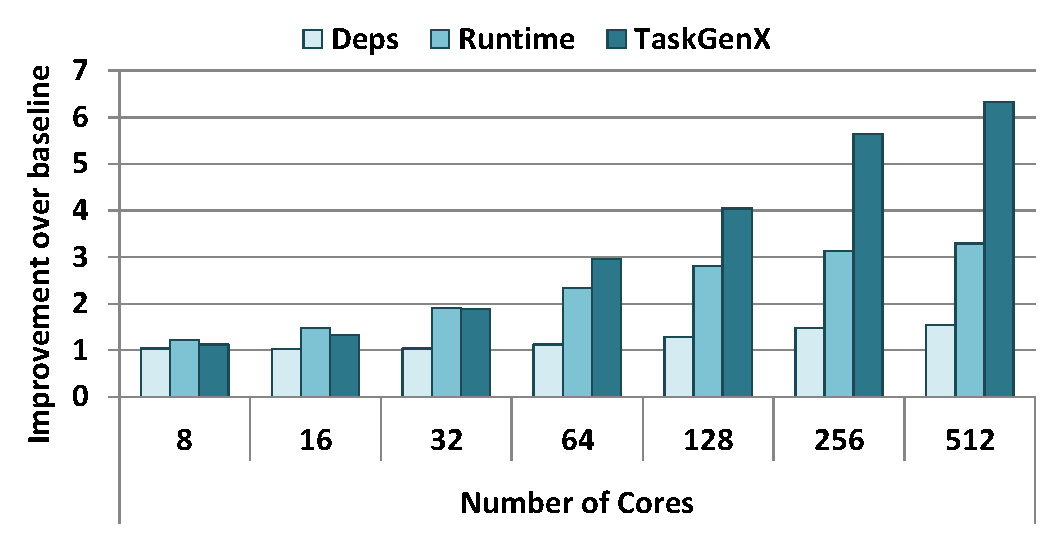
\includegraphics[width=0.75\textwidth]{figures/comparison.pdf}
	\caption{Average improvement over baseline; $x$-axis shows the number of cores.}
	\label{fig:compare}
\end{figure}
%Figure~\ref{fig:comparison} shows the average improvement for each core count over the baseline scheduler. 
As we saw earlier, {\proposal} improves the baseline scheduler by up to 6.3$\times$ for 512 cores.
In this section we compare {\proposal} with other approaches.
To do so, we consider the proposals of Carbon~\cite{Carbon}, Task Superscalar~\cite{TaskSS}, Picos++~\cite{Xubin} and Nexus\#~\cite{Nexus}.
We group these proposals based on the part of the runtime activity they are offloading from the CPU.
Carbon and Task Superscalar are runtime-driven meaning that they both accelerate all the runtime and scheduling parts.
The task creation, dependence analysis as well as the scheduling, namely the ready queue manipulation, are transferred to the RTopt with these approaches. 
These overheads are represented on Table~\ref{tab.apps} under ALL.
For the evaluation of these approaches one RTopt is used optimized to accelerate all the runtime activities. 
The second group of related designs that we compare against is the dependencies-driven, which includes approaches like Picos++ and Nexus\#. 
These approaches aim to accelerate only the dependence analysis part of the runtime as well as the scheduling that occurs when a dependency is satisfied.
The RTopt in this case is optimized to accelerate these activities.
For example, when a task finishes execution, and it has produced input for another task, the dependency tracking mechanism is updating the appropriate counters of the reader task and if the task becomes ready, the task is inserted in the ready queue.
The insertion into the ready queue is the scheduling that occurs with the dependence analysis.
These overheads are represented on Table~\ref{tab.apps} under \textit{Deps+Sched}.

%To compare {\proposal} with other systems, we emulate the behaviour of Carbon~\cite{Carbon} and Picos++~\cite{Xubin} in our system.
%In this emulation, we implement Carbon, that originally accelerates scheduling by using hardware queues. 
%To do so we decouple all the possible scheduling overheads and send them for execution by the accelerator. 
%The average per-task scheduling overheads measured are shown on Table~\ref{tab.apps} under SCHED.
%These overheads might seem high compared to the CREATE overheads that {\proposal} accelerates but they are executed among all threads so at the end they do not induce as much delay as task creation does.
%The difference between our Carbon implementation and the original one is that the original one assumes multiple hardware queues, which enables the parallel manipulation by the threads.
%In our case, we are limited to only one queue, as we want to compare an approach that would be as cheap as the {\proposal} approach and use a single hardware component.

Figure~\ref{fig:compare} shows the average improvement in performance for each core count over the performance of the baseline scheduler on the same core count. 
\textit{Runtime} represents the runtime driven approaches and the \textit{Deps} represents the dependencies driven approaches as described above.
X-axis shows the number of general purpose cores; for every core count one additional RTopt core is used.

Accelerating the scheduling with \textit{Runtime}-driven is as efficient as {\proposal} for a limited number of cores, up to 32.
This is because they both accelerate task creation which is an important bottleneck. 
\textit{Deps}-driven approaches on the other hand are not as efficient since in this case the task creation step takes place on the master thread.

Increasing the number of cores, we observe that the improvement of the \textit{Runtime}-driven over the baseline is reduced and stabilized close to 3.2$\times$ while {\proposal} continues to speedup the execution. 
Transferring all parts of the runtime to RTopt with the  \textit{Runtime}-driven approaches, leads to the serialization of the runtime.
Therefore, all scheduling operations (such as enqueue, dequeue of tasks, dependence analysis etc) that typically occur in parallel during runtime are executed sequentially on the RTopt.
Even if RTopt executes these operations faster than a general purpose core, serializing them potentially creates a bottleneck as we increase the number of cores.
{\proposal} does not transfer other runtime activities than the task creation, so it allows scheduling and dependence analysis operations to be performed in a distributed manner.

%We attribute this to the fact that serializing the scheduling operations becomes a bottleneck when increasing the number of cores.
%Scheduling operations (such as enqueue, dequeue of tasks, dependence analysis etc) generally occur in parallel during runtime, so serializing them for systems of up to 32 cores, is efficient.
%With an increased number of cores it is better to perform scheduling in a distributed manner, just as {\proposal} allows.
%
%Scheduling in general (enqueue, dequeue of tasks, dependence analysis etc) occurs in parallel during runtime.
%TaskGenX does not transfer the scheduling to the special hardware. So scheduling parts are executed on each core whenever they occur on the workers. The other approaches that do move the scheduling on the accelerator they serialize it because we assume that the accelerator is centralized. Is this clear? How could we put it clearly in the text?

%\begin{figure}[t]%
%	\centering
%	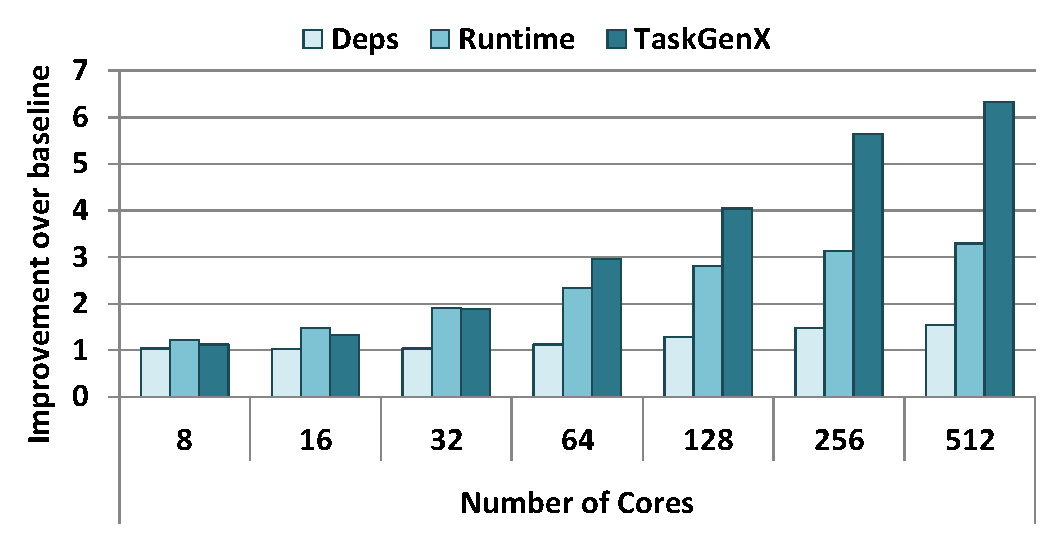
\includegraphics[width=0.6\textwidth]{figures/comparison.pdf}
%	\caption{Average improvement over baseline. X-axis shows the number of cores. For each case an RTopt core is used additionally to the number of cores.}
%	\label{fig:compare}
%	\vspace{-0.3cm}
%\end{figure}

\textit{Deps} driven approaches go through the same issue of the serialization of the dependency tracking and the scheduling that occurs at the dependence analysis stage.
The reason for the limited performance of \textit{Deps} compared to \textit{Runtime} is that \textit{Deps} does not accelerate any part of the task creation. 
Improvement over the baseline is still significant as performance with \textit{Deps} is improved by up to 1.5$\times$.

{\proposal} is the most efficient software-hardware co-design approach when it comes to highly parallel applications.
On average, it improves the baseline by up to 3.1$\times$ for homogeneous systems and up to 3.7$\times$ for heterogeneous systems.
Compared to other state of the art approaches, {\proposal} is more effective on a large number of cores showing higher performance by 54\% over \textit{Runtime} driven approaches and by 70\% over \textit{Deps} driven approaches.
